\section{Ôn tập chương}
\setcounter{section}{0}
\setcounter{subsubsection}{0}
\setcounter{ex}{0}
\setcounter{bt}{0}
 
\subsection{ĐỀ 1}
\subsubsection{Bài tập trắc nghiệm bốn phương án lựa chọn}
\begin{ex}%[Hoàng Thanh Phương]%[1D2N1-3]
	Cho dãy số $(u_n)$ với $u_n=3^n$. Số hạng thứ $n+1$ là
	\choice
	{$u_{n+1}=3^n+3$}
	{\True $u_{n+1}=3\cdot 3^n$}
	{$u_{n+1}=3^n+1$}
	{$u_{n+1}=3(n+1)$}
	\loigiai{
		Ta có $u_{n+1}=3^{n+1}=3\cdot 3^n$.\\
		Vậy số hạng thứ $n+1$ là $u_{n+1}=3\cdot 3^n$.
	}
\end{ex}
\begin{ex}%[Hoàng Thanh Phương]%[1D2H1-3]
	Cho dãy số $(u_n)$ có $u_n=\dfrac{n^2+1}{2n+1}$. Số $\dfrac{37}{13}$ là số hạng thứ bao nhiêu của dãy số đã cho?
	\choice
	{$8$}
	{\True $6$}
	{$5$}
	{$7$}
	\loigiai{
		Giả sử số hạng $u_n=\dfrac{37}{13}$ với $n\in \mathbb{N}^*$, ta có $$\dfrac{n^2+1}{2n+1}=\dfrac{37}{13}\Leftrightarrow 13n^2-74n-24=0\Leftrightarrow \hoac{& n=6 \\ 
			& n=-\dfrac{4}{13}.}$$
		Do $n\in \mathbb{N}^*$ nên $n=6$.\\
		Vậy số $\dfrac{37}{13}$ là số hạng thứ 6 dãy số $(u_n)$.
	}
\end{ex}
\begin{ex}%[Hoàng Thanh Phương]%[1D2N1-2]
	Cho dãy số: $\dfrac{1}{3}$; $\dfrac{1}{3^2}$; $\dfrac{1}{3^3}$; $\dfrac{1}{3^4}$; $\dfrac{1}{3^5}$; $\ldots$. Số hạng tổng quát của dãy số này là
	\choice
	{$u_n=\dfrac{1}{3}\cdot \dfrac{1}{3^{n+1}}$}
	{$u_n=\dfrac{1}{3^{n+1}}$}
	{\True $u_n=\dfrac{1}{3^n}$}
	{$u_n=\dfrac{1}{3^{n-1}}$}
	\loigiai{
		Dễ thấy dãy số đã cho có số hạng tổng quát là $\dfrac{1}{3^n}$.}
\end{ex}
\begin{ex}%[Hoàng Thanh Phương]%[1D2H1-5]
	Cho dãy số $(u_n)$ với $u_n=\dfrac{n+1}{n+2}$. Phát biểu nào sau đây đúng?
	\choice
	{\True Dãy số tăng và bị chặn}
	{Dãy số giảm và bị chặn}
	{Dãy số giảm và bị chặn dưới}
	{Dãy số giảm và bị chặn trên}
	\loigiai{
		Ta có\\ \centerline{$u_{n+1}-u_n=\dfrac{n+2}{n+3}-\dfrac{n+1}{n+2}=\dfrac{(n+2)(n+2)-(n+3)(n+1)}{(n+2)(n+3)}=\dfrac{1}{(n+2)(n+3)}>0,\forall n\in\mathbb{N^*}$.}
		Suy ra $\{u_n\}$ là dãy số tăng.\\
		Ta có $\dfrac{n+1}{n+2}=1-\dfrac{1}{n+2}$.\\
		Suy ra $\dfrac{2}{3}\le1-\dfrac{1}{n+2}<1$ với mọi $n\in\mathbb{N}^*$.\\
		Vậy dãy số đã cho bị chặn.
	}
\end{ex}
\begin{ex}%[Hoàng Thanh Phương]%[1D2N1-1]
	Khẳng định nào sau đây là {\bf sai}?	
	\choice
	{Một dãy số tăng thì bị chặn dưới}
	{Một dãy số giảm thì bị chặn trên}
	{\True Một dãy số bị chặn thì phải tăng hoặc giảm}
	{Một dãy số không đổi thì bị chặn}
	\loigiai{
		Dãy $(u_n)$ có $u_n=5$ với mọi $n  \in \mathbb{N}^*$ bị chặn nhưng không tăng  và không giảm.
	}
\end{ex}
\begin{ex}%[Hoàng Thanh Phương]%[1D2N2-1]
	Cho cấp số cộng $(u_n)$ có số hạng đầu $u_1$, công sai $d$. Khi đó, với $n \geq 2$ ta có
	\choice
	{$u_n=u_1+d$}
	{$u_n=u_1+(n+1) d$}
	{$u_n=u_1-(n-1) d$}      
	{\True $u_n=u_1+(n-1) d$}
	\loigiai{
		Ta có $u_n=u_1+(n-1)d$.}
\end{ex}

\begin{ex}%[Hoàng Thanh Phương]%[1D2N2-4]
	Cho cấp số cộng $(u_n)$ có $u_1=3$ và $u_2=-1$. Khi đó
	\choice
	{$u_3=4$}
	{$u_3=2$}
	{\True $u_3=-5$}
	{$u_3=7$}
	\loigiai{
		Ta có $u_2=u_1+d\Rightarrow d=u_2-u_1=-1-3=-4$.\\
		Suy ra $u_3=u_1+2d=3-8=-5$.}
\end{ex}
\begin{ex}%[Hoàng Thanh Phương]%[1D2H2-3]
	Cho cấp số cộng $(u_n)$ có số hạng đầu $u_1=-5$, công sai $d=4$. Công thức của số hạng tổng quát $u_n$ là
	\choice
	{$u_n=-5+4n$}
	{$u_n=-1-4n$}
	{$u_n=-5+4n^2$}
	{\True $u_n=-9+4n$}
	\loigiai{
		Với mọi số tự nhiên $n \ge 2$ ta có $u_n=u_1+(n-1)d=-5+(n-1)\cdot 4=4n-9$.
	}
\end{ex}
\begin{ex}%[Hoàng Thanh Phương]%[1D2H3-5]
	Có bao nhiêu số thực $x$ để $2x-1$; $x$; $2x+1$ theo thứ tự lập thành cấp số nhân?
	\choice 
	{$1$}
	{\True $2$}
	{$3$}
	{$4$}
	\loigiai{
		Vì $2x-1$; $x$; $2x+1$ theo thứ tự lập thành cấp số nhân nên $$x^2=\left(2x-1\right)\left(2x+1\right)\Leftrightarrow 3x^2-1=0\Leftrightarrow x=\pm \dfrac{1}{\sqrt{3}}.$$
	}
\end{ex}
\begin{ex}%[Hoàng Thanh Phương]%[1D2H3-4]
	Cho cấp số nhân $(u_n)$ có $u_1=-1$, công bội $q=-\dfrac{1}{10}$. Khi đó $\dfrac{1}{10^{2017}}$ là số hạng thứ mấy?
	\choice
	{$2016$}
	{$2017$}
	{\True $2018$}
	{$2019$}
	\loigiai{
		Ta có số hạng tổng quát của dãy số là $u_n=u_1\cdot q^{n-1}=\left(-1\right)\cdot \left(-\dfrac{1}{10}\right)^{n-1}$.\\
		Giả sử $\dfrac{1}{10^{2017}}$ là số hạng thứ $n$ của cấp số nhân, ta có $$u_n=\dfrac{1}{10^{2017}}  \Leftrightarrow (-1)\cdot \left(-\dfrac{1}{10}\right)^{(n-1)}=\dfrac{1}{10^{2017}} \Leftrightarrow n=2018.$$
	}
\end{ex}
\begin{ex}%[Hoàng Thanh Phương]%[1D2H2-6]
	Tổng của $100$ số tự nhiên lẻ đầu tiên tính từ $1$ là
	\choice
	{\True $10000$}
	{$10100$}
	{$20000$}
	{$20200$}
	\loigiai{
		Ta có $100$ số lẻ đầu tiên tạo thành cấp số cộng có $100$ số hạng với $u_1=1$, $d=2$ và $u_{100}=199$.\\
		Tổng $n$ số lẻ đầu tiên là $S_{100}=\dfrac{\left(u_1+u_{100}\right)\cdot 100}{2}=10000$.	
	}
\end{ex}
\begin{ex}%[Hoàng Thanh Phương]%[1D2H2-7]
	Một gia đình cần khoan một cái giếng để lấy nước. Họ thuê một đội khoan giếng nước đến để khoan giếng. Biết giá của mét khoan đầu tiên là $80\,000$ đồng, kể từ mét khoan thứ hai giá của mỗi mét khoan tăng thêm $5000$ đồng so với giá của mét khoan trước đó. Biết cần phải khoan sâu xuống $50$ m mới có nước. Hỏi phải trả bao nhiêu tiền để khoan cái giếng đó?
	\choice 
	{\True $10\, 125\,000$ đồng}
	{$5\, 250\,000$ đồng}
	{$4\, 245\,000$ đồng}
	{$4\, 000\,000$ đồng}
	\loigiai{
		Số tiền phải trả ở mỗi mét khoan tạo thành một cấp số cộng có số hạng đầu $u_1 = 80\,000$ và công sai $d=5000$.\\
		Như vậy, tổng số tiền khi khoan đến mét thứ $n$ được tính theo công thức
		$$S_n=\dfrac{n}{2}\left[2u_1+(n-1)d\right].$$
		Vậy tổng số tiền phải trả là 
		$$S_{50}=25\cdot \left( 2\cdot 80\,000+ 49\cdot 5000\right)=10\,125\,000.$$
	}
\end{ex}
\subsubsection{Bài tập trắc nghiệm đúng sai}
\begin{ex}%[Hoàng Thanh Phương]%[1D2V1-5]
	Cho dãy số $u_n=\dfrac{2n+1}{n+3},~\forall n\in\mathbb{N}^*$. Các khẳng định sau là đúng hay sai?
	\choiceTF[t]
	{\True $u_3=\dfrac{7}{6}$}
	{\True $u_n<2,~\forall n\in\mathbb{N}^*$}
	{Dãy số trên là dãy số giảm}
	{\True Dãy số trên là dãy số bị chặn}
	\loigiai{
	\begin{itemchoice}
		\itemch Ta có $u_3=\dfrac{2\cdot 3+1}{3+3}=\dfrac{7}{6}$. \\
		Khẳng định trên là đúng.
		\itemch Ta có $u_n=\dfrac{2n+1}{n+3}<\dfrac{2n+6}{n+3}=2$. Vậy $u_n<2,~\forall n\in\mathbb{N}^*$. \\
		Khẳng định trên là đúng.
		\itemch Ta có $u_1=\dfrac{3}{4}$, $u_2=1$. \\
		Ta có $u_{n+1}=\dfrac{2n+3}{n+4}$, $u_{n+1}-u_n=\dfrac{2n+3}{n+4}-\dfrac{2n+1}{n+3}=\dfrac{5}{(n+4)(n+3)}>0,~\forall n\in\mathbb{N}^*$. \\
		Vậy $u_{n+1}>u_n~\forall n\in\mathbb{N}^*$, nên dãy đã cho là dãy tăng. \\
		Khẳng định trên là sai.
		\itemch Ta có $n\in\mathbb{N}^*$ nên $u_n=\dfrac{2n+1}{n+3}>0$. \\
		Mặt khác, ta đã chứng minh $u_n<2~\forall n\in\mathbb{N}^*$. \\
		Vậy $0<u_n<2$, nên dãy số đã cho là dãy bị chặn. Khẳng định trên là đúng.
	\end{itemchoice}	
}
\end{ex}
\begin{ex}%[Hoàng Thanh Phương]%[1D2V2-6]
	Cho cấp số cộng $\left(u_n\right)$ có số hạng đầu $u_1=-5$ và công sai $ d=3$.
	\choiceTF[t]
	{\True Số $100$ là số hạng thứ $36$ của cấp số cộng}
	{ Số hạng thứ $5$ của cấp số cộng là $ 9$}
	{\True Tổng $10$ số hạng đầu của cấp số cộng là $85$}
	{Số hạng tổng quát của cấp số cộng $\left(u_n\right)$ là $\left(u_n\right)=3n-7$}
	\loigiai{
		\begin{itemchoice} 
			\itemch Ta có
			$u_n=u_1+(n-1)d\Leftrightarrow 100=-5+(n-1)3\Leftrightarrow n=36$. \\
			Khẳng định trên là đúng.
			\itemch Ta có $u_5=u_1+4d=-5+4\cdot3=7$. \\
			Khẳng định trên là sai.
			\itemch Ta có
			$S_n=\dfrac{n}{2}\left[2u_1+(n-1)d\right]\Rightarrow{S_{10}}=\dfrac{10}{2}\left[2\cdot(-5)+(10-1)3\right]=85$. \\
			Khẳng định trên là đúng.
			\itemch $u_n=u_1+\left(n-1\right)d=-5+\left(n-1\right)3=3n-8$. \\
			Khẳng định trên là sai.
	\end{itemchoice}}
\end{ex}
\begin{ex}%[Hoàng Thanh Phương]%[1D2V2-7]
	Một gia đình mua một chiếc ô tô giá $800$ triệu đồng. Trung bình sau mỗi năm sử dụng, giá trị còn lại của ô tô giảm đi $4 \%$ (so với năm trước đó). Các khẳng định sau là đúng hay sai?
	\choiceTF[t]
	{\True Giá trị còn lại của ô tô sau từng năm lập thành một cấp số nhân với công bội nhỏ hơn $1$}
	{Giá trị của chiếc xe sau $3$ năm  gần bằng $508{,}84$ triệu đồng}
	{\True Giá trị của chiếc xe sau $5$ năm lớn hơn một nửa giá trị ban đầu của chiếc xe}
	{Nếu sau một thời gian sử dụng, gia đình muốn bán lại chiếc xe để thu được ít nhất $600$ triệu đồng thì gia đình đó nên sử dụng ít hơn $6$ năm}
	\loigiai{
		Sau mỗi năm, giá trị của chiếc xe bằng $96\%$ giá trị của năm ngoái, vậy giá trị chiếc xe lập thành một cấp số nhân với $u_1=800$ và $q=0{,}96$. \\
		Giá trị chiếc xe sau $n$ năm là $u_n=800\cdot (0{,}96)^n$.
		\begin{itemchoice}
			\itemch Khẳng định trên là đúng.
			\itemch Ta có $u_n=800\cdot (0{,}96)^{n}$. \\
			Giá trị của chiếc xe sau $3$ năm là $u_3=800\cdot (0{,}96)^3a\approx 707{,}79$ (triệu đồng). \\
			Khẳng định trên là sai.
			\itemch Giá trị của chiếc xe sau $5$ năm là  $u_5=800\cdot (0{,}96)^5\approx 652{,}3$ (triệu đồng). \\
			Khẳng định trên là đúng.
			\itemch Ta có $u_7\approx 601{,}16$ và $u_8\approx 577{,}11$ triệu đồng. \\
			Vậy gia đình muốn bán lại chiếc xe để thu được ít nhất $600$ triệu đồng thì gia đình đó nên dùng chiếc xe ít hơn $7$ năm.
		\end{itemchoice}	
	}
\end{ex}
\begin{ex}%[Hoàng Thanh Phương]%[1D2H2-6]
	Cho một cấp số cộng $\left(u_n\right)$ có $u_1=\dfrac{1}{3}$, $u_8=26$, có công sai $d$.
	\choiceTF[t]
	{\True $d=\dfrac{11}{3}$}
	{\True $u_{11}=37$}
	{Tổng $102$ số hạng đầu của dãy số là $S_{102}=\dfrac{1124}{3}$}
	{Trong $100$ số hạng đầu tiên của dãy số $(u_n)$, có đúng $34$ số hạng là số nguyên}
	\loigiai{
		\begin{itemchoice}
			\itemch Ta có $\heva{&u_1=\dfrac{1}{3}\\&u_8=26}\Leftrightarrow \heva{&u_1=\dfrac{1}{3}\\&u_1+7d=26}\Leftrightarrow \heva{&u_1=\dfrac{1}{3}\\&d=\dfrac{11}{3}.}$ \\
			Vậy $d=\dfrac{11}{3}$.
			\itemch $u_{11}=u_1+10d=37$.
			\itemch Ta có $S_{102}=2u_1 + 101d=371$.
			\itemch Vì $u_n=u_1 + (n-1)d=\dfrac{11n-10}{3}$ nên $u_n$ là số nguyên khi $11n-10$ chia hết cho $3$.\\
			Mà $11n-10=(9n-9)+(2n-1)$ nên $u_n$ là số nguyên khi $2n-1$ chia hết cho $3$, với $n\in\{1;\ldots;100\}$.\\
			Suy ra $n\in \{2;5;8;\ldots;98\}$, do đó có đúng $\dfrac{98-2}{3}+1=33$ số hạng đầu tiên của dãy số $(u_n)$ là số nguyên.
		\end{itemchoice}
	}
\end{ex}
\subsubsection{Bài tập trắc nghiệm trả lời ngắn}
\begin{ex}%[Hoàng Thanh Phương]%[1D2H2-7]
	Người ta trồng cây theo các hàng ngang với quy luật: ở hàng thứ nhất có $1$ cây, ở hàng thứ hai có $2$ cây, ở hàng thứ ba có $3$ cây, $\ldots$ ở hàng thứ $n$ có $n$ cây. Biết rằng người ta trồng hết $4950$ cây. Hỏi số hàng cây được trồng theo cách trên là bao nhiêu?
	\shortans{100}
	\loigiai{
		Số cây ở mỗi hàng lập thành một cấp số cộng với $u_1=1$ và công sai $d=1$.\\
		Theo giả thiết Ta có $S_n=4950 \Leftrightarrow n+\dfrac{(n-1)n}{2} =4950  \Leftrightarrow n^2 +n -4950=0 \Leftrightarrow \hoac{&n=-99 \text{ (loại)}\\&n=100.}$\\
		Vậy có $100$ hàng cây được trồng.
	}
\end{ex}
\begin{ex}%[Hoàng Thanh Phương]%[1D2H2-7]
	Một du khách vào chuồng đua ngựa đặt cược, lần đầu tiên đặt $20$ ngàn đồng, mỗi lần sau tiền đặt gấp đôi lần tiền đặt cược trước. Người đó thua lần $9$ liên tiếp và thắng ở lần thứ $10$. Hỏi cuối cùng du khách đó thắng hay thua bao ngàn đồng (quy ước số tiền thắng mang dấu dương và số tiền thua mang dấu âm).
	\shortans{20}
	\loigiai{
		Số tiền đặt cược lần thứ $n$ là $u_n=u_1\cdot 2^{n-1}$ với $u_1=20000$. \\
		Số tiền người khách đó thắng cược ở lần thứ $10$ là $20000\cdot 2^9$. \\
		Số tiền người khách đó thua ở $9$ lần trước là $\displaystyle\sum_{n=1}^9 20000\cdot 2^{n-1}$. \\
		Vậy số tiền người khách đó thu được sau ván cược thứ $10$ là $$u_{10}-\displaystyle\sum_{n=1}^9 u_1\cdot 2^{n-1}=20000\cdot 2^9-\displaystyle\sum_{n=1}^9 20000\cdot 2^{n-1}=20000.$$
		Vậy du khách thắng $20000$ đồng.
	}
\end{ex}
\begin{ex}%[Hoàng Thanh Phương]%[1D2H2-7]
	Một người gửi ngân hàng 100 triệu đồng với kỳ hạn 3 tháng, lãi suất $2\%$ một quý theo hình thức lãi kép. Sau đúng 6 tháng, người đó gửi thêm 100 triệu đồng với kỳ hạn và lãi suất như trước đó. Tổng số tiền người đó nhận được sau 1 năm kể từ khi bắt đầu gửi tiền gần bằng bao nhiêu triệu đồng (làm tròn kết quả tới hàng đơn vị)?
	\shortans{212}
	\loigiai{
		Số tiền người đó nhận được sau 6 tháng đầu: $100\cdot(1+2\%)^2$.\\
		Số tiền người đó nhận được sau 6 tháng tiếp theo là: $\left[100\cdot(1+2\%)^2+100\right]\cdot(1+2\%)^2\approx 212{,}28$.
	}
\end{ex}
\begin{ex}%[Hoàng Thanh Phương]%[1D2V2-7]
	Một cái tháp có $11$ tầng. Diện tích của mặt sàn tầng $2$ bằng nửa diện tích của mặt đáy tháp và diện tích của mặt sàn mỗi tầng bằng nửa diện tích của mặt sàn mỗi tầng ngay bên dưới. Biết mặt đáy tháp có diện tích là $12 288$ m$^2$. Tính diện tích của mặt sàn tầng trên cùng của tháp theo đơn vị mét vuông.
	\shortans{12}
	\loigiai{
		Do diện tích của mặt sàn tính từ tầng một lập thành một cấp số nhân với $u_2=\dfrac{1}{2}\cdot 12288=6144$ và $q=\dfrac{1}{2}$.\\
		Ta có $\heva{u_2&=6144 \\ q&=\dfrac{1}{2}}  \Leftrightarrow \heva{u_1&=12288 \\ q&=\dfrac{1}{2}.}$\\
		Ta có $u_{11}=u_1\cdot q^{10}=12288\cdot \dfrac{1}{12^{10}}=12$m$^2$.\\
		Vậy diện tích của mặt sàn tầng trên cùng là	$12$ m$^2$.
	}
\end{ex}
\begin{ex}%[Hoàng Thanh Phương]%[1D2V2-7]
	Từ độ cao $55{,}8$ (mét) của tháp nghiên Pisa nước Italia người ta thả một quả bóng cao su chạm xuống đất. Giả sử mỗi lần chạm đất bóng lại nảy lên độ cao bằng $\dfrac{1}{10}$ độ cao mà bóng đạt trước đó. Tổng độ dài hành trình (mét) của bóng được thả từ lúc ban đầu cho đến khi nó nằm yên trên mặt đất gần bằng bao nhiêu (làm tròn đến chữ số thập phân thứ nhất)?
	\shortans{68,2}
	\loigiai{
		Đặt $u_1=55{,}8$ (mét) là quãng đường bóng rơi khi thả xuống, $u_{n+1}=\dfrac{1}{10^{n}} u_1, n\ge 1$ là quãng đường bóng rơi sau lần nảy lên thứ $n$. \\ 
		Ta có $(u_n)$ là dãy cấp số nhân với $u_1=55{,}8$ và công bội $q=\dfrac{1}{10}$.\\ 
		Suy ra tổng quãng đường quả bóng rơi xuống là $\displaystyle \lim \limits_{n \rightarrow +\infty} u_1 \cdot \dfrac{1-q^n}{1-q}=\displaystyle \lim \limits_{n \rightarrow +\infty}55{,}8\cdot\dfrac{1-\left( \dfrac{1}{10}\right)^n}{1-\dfrac{1}{10}}=62 $.	\\ 
		Ngoài ra ta còn phải tính tổng quãng đường mà bóng nảy lên. Ta có tổng quãng đường bóng nảy lên bằng tổng quãng đường rơi của bóng trừ đi quãng đường thả rơi xuống.\\ 
		Vậy tổng quãng đường hành trình của quả bóng là $62+62-55{,}8=68{,}2$ (mét).	
	}
\end{ex}
\begin{ex}%[Hoàng Thanh Phương]%[1D2C2-7]
	\immini{
		Cho hình vuông $ABCD$ có các cạnh bằng a và có diện tích $S_1$.
		Nối 4 trung điểm $A_1,B_1,C_1,D_1$ theo thứ tự của 4 cạnh $AB, BC, CD, DA$ 
		ta được hình vuông thứ hai có diện tích $S_2$. Tiếp tục làm như thế,
		ta được hình vuông thứ ba là $A_2,B_2,C_2,D_2$ có diện tích $S_3$,...
		và cứ tiếp tục làm như thế, ta tính được các hình vuông lần lượt
		có diện tích có diện tích $S_4,S_5,\ldots,S_{100}$ (tham khảo hình vẽ bên).
		Giá trị tổng có diện tích $S=S_1+S_2+S_3+ \cdots +S_{100}$ là $\dfrac{a^m(2^{n}-1)}{2^{p}}$, với $m, n, p\in\mathbb{N}^*$. Tính giá trị biểu thức $T=m+n-p$.
		\shortans{3}
	}{	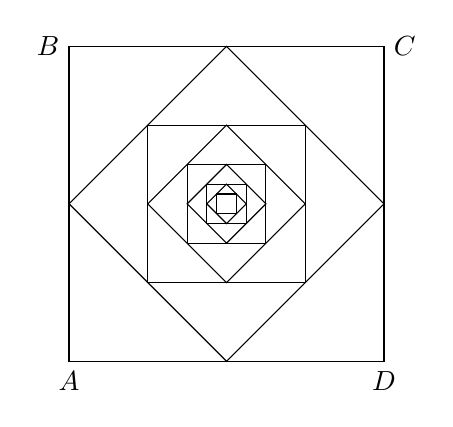
\begin{tikzpicture}
			\def\a{2} %cạnh hình vuông
			\def\t{.5} % tỷ lệ điểm cho vòng lặp tiếp
			\path
			(-\a,-\a) coordinate (A1)node[below]{$A$}
			(-\a,\a) coordinate (B1)node[left]{$B$}
			(\a,\a) coordinate (C1)node[right]{$C$}
			(\a,-\a) coordinate (D1)node[below]{$D$};
			\draw (A1)--(B1)--(C1)--(D1)--cycle;
			\foreach \i[count=\j from 2] in {1,...,8}
			\draw
			(barycentric cs:A\i=\t,B\i=1-\t) coordinate (A\j)--
			(barycentric cs:B\i=\t,C\i=1-\t) coordinate (B\j)--
			(barycentric cs:C\i=\t,D\i=1-\t) coordinate (C\j)--
			(barycentric cs:D\i=\t,A\i=1-\t) coordinate (D\j)--cycle
			;
	\end{tikzpicture}}
	\loigiai{
		Ta có $S_1=a^2;S_2=\dfrac{1}{2}a^2;S_3=\dfrac{1}{4}a^2, \ldots$ \\
		Do đó $S_1,S_2,S_3,\ldots,S_{100}$ là cấp số nhân với số hạng đầu $u_1=S_1=a^2$ và công bội $q=\dfrac{1}{2}$.\\
		Suy ra $S=S_1+S_2+S_3+ \cdots +S_{100}=S_1 \cdot \dfrac{1-q^n}{1-q}=\dfrac{a^2(2^{100}-1)}{2^{99}}$.
Vậy $m+n-p=2+100-99=3$.
}
\end{ex}
